\documentclass{beamer}

\usepackage[utf8]{inputenc}
%\usepackage{default}

\usetheme{Berlin}

\title{Imagerie Médicale}
\subtitle{Ingénierie d'une application}
%\author{Jérôme Velut}
\date{04/12/2013}

\begin{document}

\frame{\titlepage}

\section*{Sommaire}
\begin{frame}{Sommaire}
  \tableofcontents[hideallsubsections]
\end{frame}

\section{Imagerie médicale}
\subsection{Bref historique}
\begin{frame}{Médecine nucléaire}
\begin{columns}[T]
 \begin{column}{0.5\textwidth}
 \centering
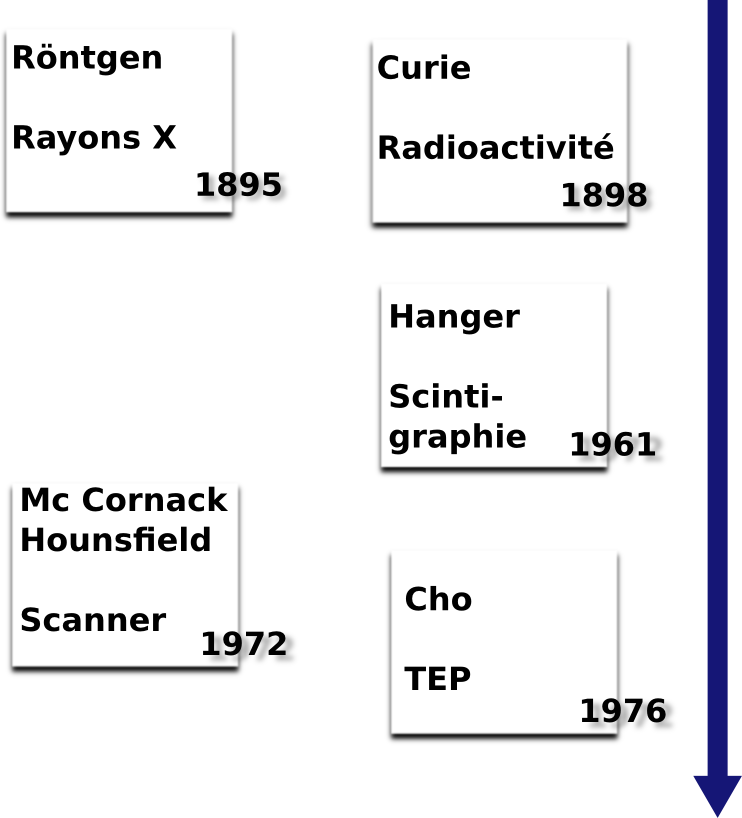
\includegraphics[height=0.7\textheight]{images/historique_radio.png}
 \end{column}
 \begin{column}{0.5\textwidth}
\begin{itemize}
 \item Médecine nucléaire: imageries, traitements par rayonnement ionisant
 \item Applications industrielles également
 \item Effets sur la santé
\end{itemize}
 \end{column}
\end{columns}
\end{frame}
\begin{frame}{Médecine nucléaire}
\begin{columns}[T]
 \begin{column}{0.5\textwidth}
 \centering
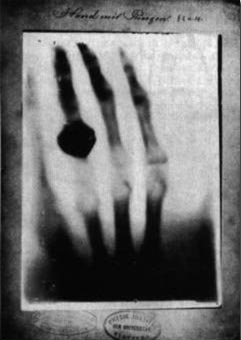
\includegraphics[height=0.7\textheight]{images/main_roentgen.jpg}\\
Première radiographie
 \end{column}
 \begin{column}{0.5\textwidth}
 \centering
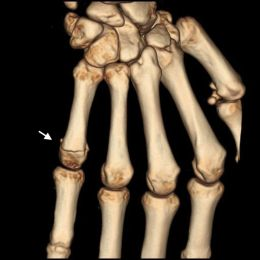
\includegraphics[height=0.5\textheight]{images/main_TDM.jpg}\\
Scanner haute résolution (fracture)
 \end{column}
\end{columns}
\end{frame}
\begin{frame}{Résonance magnétique}
\begin{columns}[T]
 \begin{column}{0.5\textwidth}
 \centering
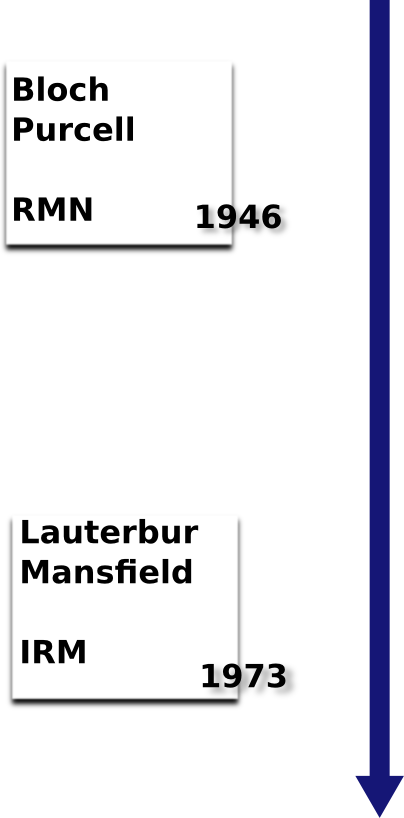
\includegraphics[height=0.7\textheight]{images/historique_rmn.png}
 \end{column}
 \begin{column}{0.5\textwidth}
\begin{itemize}
 \item Emission d'une onde radiofréquence par les noyaux placés dans un champ magnétique
 \item Spectroscopie RMN : observation de différents isotopes
 \item IRM: observation de l'hydrogène
\end{itemize}
 \end{column}
\end{columns} 
\end{frame}
\begin{frame}{Résonance magnétique}
\begin{columns}[T]
 \begin{column}{0.5\textwidth}
 \centering
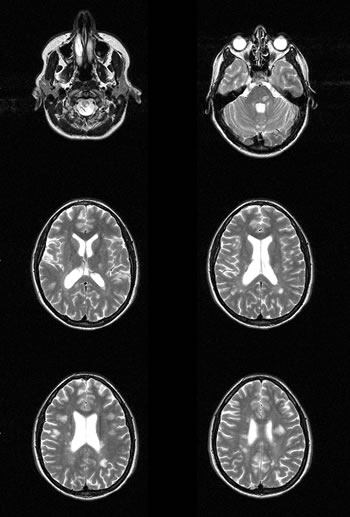
\includegraphics[height=0.6\textheight]{images/irm_t2.jpg}\\
IRM pondération T1
 \end{column}
 \begin{column}{0.5\textwidth}
 \centering
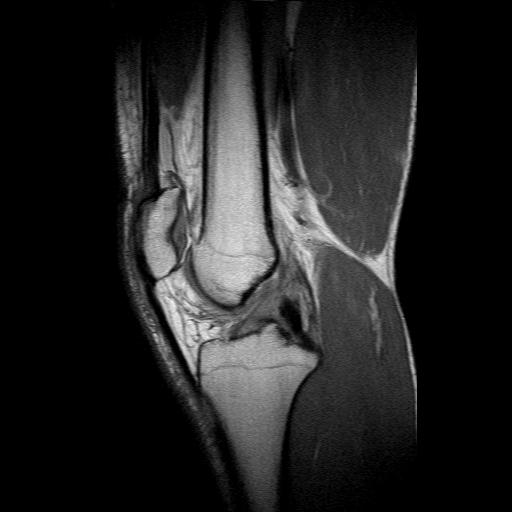
\includegraphics[height=0.6\textheight]{images/IRM_genou_sag_2.png}\\
IRM pondération T2
 \end{column}
\end{columns} 
\end{frame}

\begin{frame}{Ultrasons}
 \begin{columns}[T]
 \begin{column}{0.5\textwidth}
 \centering
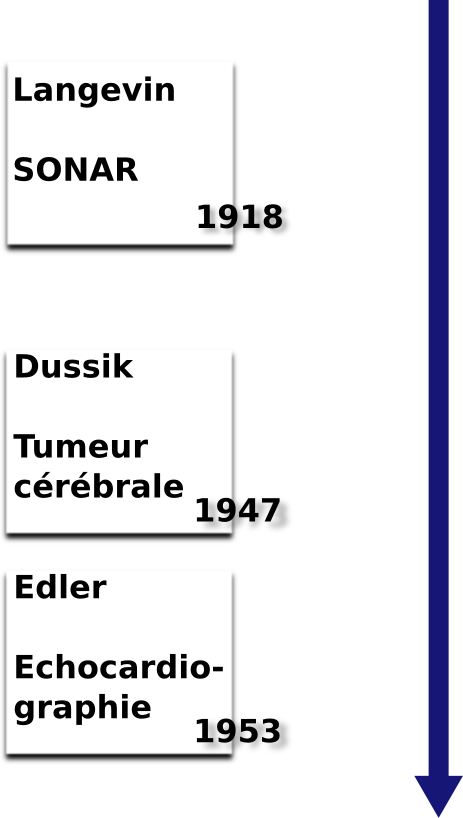
\includegraphics[height=0.7\textheight]{images/historique_us.png}
 \end{column}
 \begin{column}{0.5\textwidth}
\begin{itemize}
 \item Mesure la reflexion des ondes ultrasonores
 \item Effet Doppler : mesure de vitesse
 \item Portable, non invasif, innocuité++
\end{itemize}
 \end{column}
\end{columns} 
\end{frame}
\begin{frame}{Ultrasons}
 \begin{columns}[T]
 \begin{column}{0.32\textwidth}
 \centering
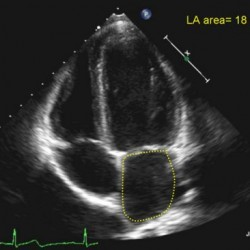
\includegraphics[width=0.9\textwidth]{images/echocardio.jpg}\\
Echographie cardiaque
 \end{column}
 \begin{column}{0.32\textwidth}
 \centering
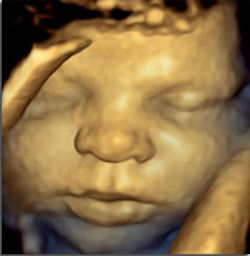
\includegraphics[width=0.9\textwidth]{images/echo3d.jpg}\\
Obstétrique
 \end{column}
 \begin{column}{0.32\textwidth}
 \centering
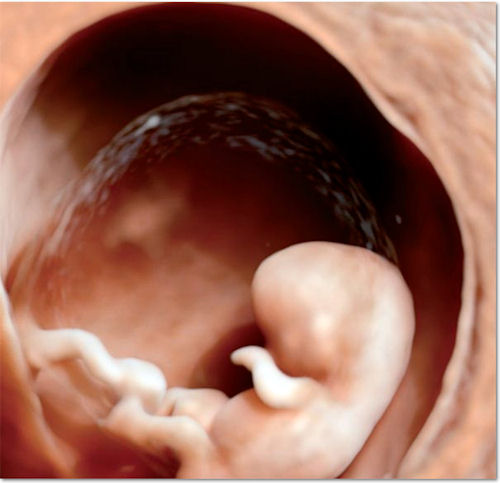
\includegraphics[width=0.9\textwidth]{images/echo3dhd.jpg}\\
Avec un bon traitement d'image...
 \end{column}\end{columns} 
\end{frame}
\subsection{Méthodes de diagnostic}
\begin{frame}{Diagnostic}
\begin{itemize}
 \item Diagnostic = identifier les causes des symptômes (étiologie) en vue d'adapter le traitement
 \item US, IRM, TDM: imagerie anatomique (ou structurelle)
 \item USf, IRMf, TEP: imagerie fonctionnelle
 \item Rôle de l'imagerie: exploration - décision
\end{itemize}
\end{frame}

\begin{frame}{Diagnostic}
  \begin{columns}[t]
 \begin{column}{0.5\textwidth}
 \begin{block}{Exploration}
  \begin{itemize}
   \item Recherche de pathologies
   \item $\rightarrow$ Segmentations
   \item $\rightarrow$ Interactions
  \end{itemize}
 \end{block}
 \end{column}
 \begin{column}{0.5\textwidth}
 \begin{block}{Décision}
  \begin{itemize}
   \item Adaptation du traitement
   \item $\rightarrow$ Quantifications
  \end{itemize}
 \end{block}
\end{column}
\end{columns}
\end{frame}

\subsection{Thérapie guidée par l'image}
\begin{frame}{Principes}
\centering
  \begin{columns}[t]
 \begin{column}{0.5\textwidth}
\begin{block}{Améliorer la précision}
\begin{itemize}
  \item localisation
  \item dose
 \end{itemize}
\end{block}
 \end{column}
 \begin{column}{0.5\textwidth}
\begin{block}{Diminuer les traumatismes}
\begin{itemize}
  \item Interventions non (mini) invasives
  \item gestes chirurgicaux plus rapides
  \end{itemize}
\end{block}
\end{column}
\end{columns}
  (\small$\rightarrow$ robotique médicale)
\end{frame}
\begin{frame}{Planification}
 \centering
  \begin{columns}[t]
 \begin{column}{0.5\textwidth}
\begin{block}{Planification}
\begin{itemize}
 \item Prévoir l'intervention (par ex. dépôt de dose)
 \item Imagerie anatomique et/ou fonctionnelle : localisation
 \item Modification topologique lors de l'intervention
\end{itemize}\end{block}
 \end{column}
 \begin{column}{0.5\textwidth}
\begin{block}{Guidage par l'image}
\begin{itemize}
  \item Modification de la planification en cours de traitement
  \item $\rightarrow$ Moins de traitement
  \item $\rightarrow$ Plus efficace
  \end{itemize}
\end{block}
\end{column}
\end{columns}
\end{frame}

\begin{frame}{Couplages}
 \centering
  \begin{columns}[T]
 \begin{column}{0.5\textwidth}
\begin{block}{CBCT/Radiotherapie}
\begin{itemize}
 \item Recalage 2D/3D (CBCT vs. CT référence)
 \item Localisation précise des doses
 \item Utilisation per-opératoire
\end{itemize}
\end{block}
 \end{column}
 \begin{column}{0.5\textwidth}
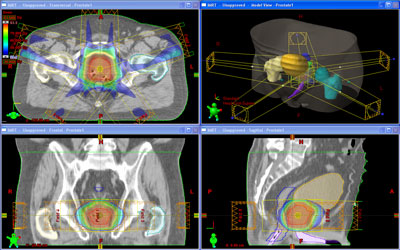
\includegraphics[width=0.9\textwidth]{images/cbct_radio.jpg}
\end{column}
\end{columns}
\end{frame}
\begin{frame}{Couplages}
 \centering
  \begin{columns}[T]
 \begin{column}{0.5\textwidth}
\begin{block}{PET/CT}
\begin{itemize}
 \item Localisation des sources
 \item Planification uniquement
 \item Utilisation per-operatoire en discussion
\end{itemize}
\end{block}
 \end{column}
 \begin{column}{0.5\textwidth}
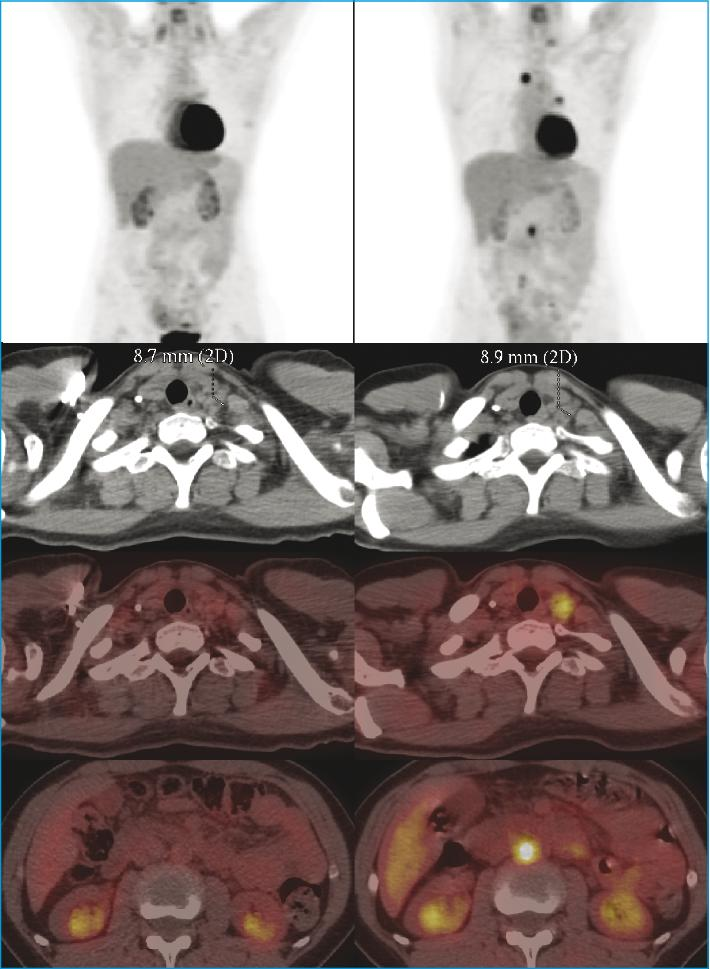
\includegraphics[height=0.7\textheight]{images/pet_ct.jpg}
\end{column}
\end{columns}
\end{frame}

\begin{frame}{Couplages}
 \centering
  \begin{columns}[T]
 \begin{column}{0.5\textwidth}
\begin{block}{Ultrasons/HIFU}
\begin{itemize}
  \item Image écho
  \item traitement HIFU
  \item Même système image et traitement
  \end{itemize}
\end{block}
 \end{column}
 \begin{column}{0.5\textwidth}
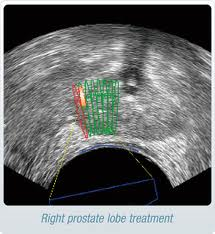
\includegraphics[height=0.5\textheight]{images/hifu_echo.jpg}
\end{column}
\end{columns}
\end{frame}

\subsection{Thérapie par ultrasons focalisés de haute intensité}
\begin{frame}{Indications}
  \centering
  \begin{columns}[T]
 \begin{column}{0.5\textwidth}
\begin{block}{Pathologie}
\begin{itemize}
  \item Cancer de la prostate
  \item Traitement complet ou localisé de la glande
  \item Cancer moyennement agressif (gleason$<$7)
  \end{itemize}
\end{block}
 \end{column}
 \begin{column}{0.5\textwidth}
\begin{block}{Avantage}
\begin{itemize}
  \item Préservation de la qualité de vie (continence et fonction érectile)
  \item Traitement d'une récidive
  \end{itemize}
\end{block}
\end{column}
\end{columns}
\end{frame}

\begin{frame}{Technologie}
  \centering
  \begin{columns}[T]
 \begin{column}{0.5\textwidth}
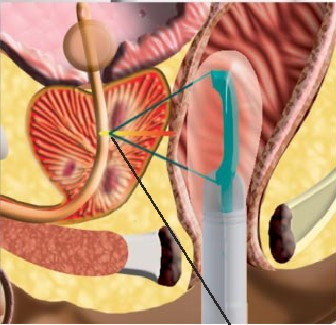
\includegraphics[height=0.5\textheight]{images/hifu.jpg}
 \end{column}
 \begin{column}{0.5\textwidth}
\begin{block}{Ablathermie}
\begin{itemize}
  \item Chirurgie destructrice
  \item Augmentation de la temperature des tissus
  \end{itemize}
\end{block}
\begin{block}{Traitement focal}
\begin{itemize}
  \item Cible les tissus pathologiques
  \item Réduit les marges de sécurité
  \end{itemize}
\end{block}
\end{column}
\end{columns}
 
\end{frame}

\begin{frame}{Apport de l'IRM}
  \centering
  \begin{columns}[T]
 \begin{column}{0.5\textwidth}
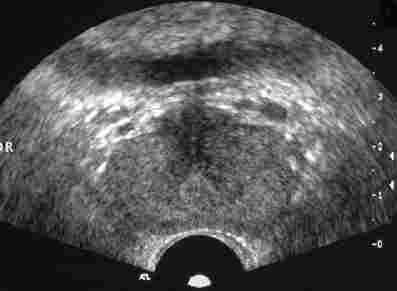
\includegraphics[height=0.5\textheight]{images/echo_prostate.jpg}
 \end{column}
 \begin{column}{0.5\textwidth}
\begin{block}{Echographie prostatique}
\begin{itemize}
  \item Proximité des organes à risque
  \item Où est la tumeur ?
  \end{itemize}
\end{block}
\end{column}
\end{columns} 
\end{frame}

\begin{frame}{Apport de l'IRM}
  \centering
  \begin{columns}[T]
 \begin{column}{0.5\textwidth}
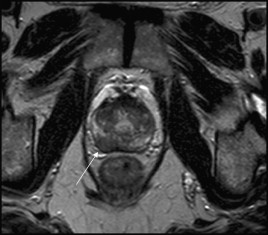
\includegraphics[height=0.5\textheight]{images/irm_prostate.jpg}
 \end{column}
 \begin{column}{0.5\textwidth}
\begin{block}{IRM T2}
\begin{itemize}
  \item Antenne de surface
  \item Tumeur localisée par le radiologue
  \end{itemize}
\end{block}
\end{column}
\end{columns} 
\end{frame}

\begin{frame}{Apport de l'IRM}
  \centering
Collaboration urologue/radiologue
  \begin{columns}[T]
 \begin{column}{0.5\textwidth}
\begin{block}{Radiologue}
\begin{itemize}
  \item Phase de planification
  \item Localise la prostate sur l'IRM
  \item Localise la tumeur sur l'IRM
  \end{itemize}
\end{block}
 \end{column}
 \begin{column}{0.5\textwidth}
\begin{block}{Urologue}
\begin{itemize}
  \item Planification: quantification
  \item Traitement à partir... des images écho
  \end{itemize}
\end{block}
\end{column}
\end{columns}
\begin{exampleblock}{Besoin}
Mise en correspondance des images écho et IRM.
\end{exampleblock}
\end{frame}

\section{Recalage d'images}
\subsection{Objectifs}
\begin{frame}{Mise en correspondance}
  \begin{columns}[T]
 \begin{column}{0.5\textwidth}
\begin{block}{Contexte}
\begin{itemize}
  \item Acquisitions différentes
  \item Mono-modalité : suivi longitudinale
  \item Multi-modalité : fusion d'information
  \end{itemize}
\end{block}
 \end{column}
 \begin{column}{0.5\textwidth}
\begin{block}{Mise en correspondance}
\begin{itemize}
  \item Minimisation de la différence
  \item Maximisation de la similarité
  \item $\rightarrow$ Transformation optimale
  \end{itemize}
\end{block}
\end{column}
\end{columns}
\end{frame}

\begin{frame}{Mise en correspondance}
  \begin{columns}[T]
 \begin{column}{0.5\textwidth}
\begin{block}{Pré-acquisition}
\begin{itemize}
  \item Connaissance a priori de la géométrie
  \item Contraintes physiques sur le patient
  \item Intégration de modalités différentes
  \end{itemize}
\end{block}
 \end{column}
 \begin{column}{0.5\textwidth}
\begin{block}{Post-acquisition}
\begin{itemize}
  \item Traitement d'image (recalage)
  \item Estimation de la transformation optimale
  \item Image fixe/image mobile
  \end{itemize}
\end{block}
\end{column}
\end{columns}
\end{frame}

\subsection{Méthode}
\begin{frame}{Vue globale}
\centering
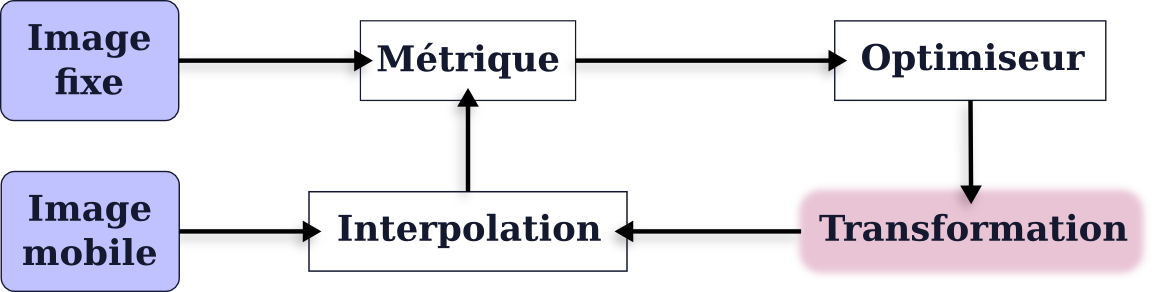
\includegraphics[width=0.7\textwidth]{images/recalage.png}\\
Algorithme de recalage : {\bfseries transformation} de l'image mobile permettant d'optimiser une métrique liée à l'image fixe. 
\end{frame}
\begin{frame}{Métrique}
   \begin{columns}[T]
 \begin{column}{0.5\textwidth}
\begin{block}{Quel repère?}
\begin{itemize}
  \item Image ? (indice de pixel)
  \item Environnement 3D ? (coordonnées cartésiennes)
  \item $\rightarrow$ Interpolation
  \end{itemize}
\end{block}
 \end{column}
 \begin{column}{0.5\textwidth}
\begin{block}{Quelle mesure?}
\begin{itemize}
  \item $\mathcal{F}(I_f, T(I_m))$
  \item dépend de la nature des images
  \end{itemize}
\end{block}
\end{column}
\end{columns}
\end{frame}
\begin{frame}{Métrique}
\centering
   \begin{columns}[c]
 \begin{column}{0.5\textwidth}
\begin{block}{Le classique: MSE}
\begin{itemize}
  \item différence pixel à pixel, au carré, sommée
  \item 2 images identiques ont une MSE nulle
  \item Rapide, efficace, mais...
  \end{itemize}
\end{block}
 \end{column}
 \begin{column}{0.5\textwidth}
$\mathcal{F}(I_f, T(I_m)) = \sum{(I_f(i)-T(I_m)(i))^2}$
\end{column}
\end{columns}
\end{frame}
\subsection{Recalage multimodal}
\begin{frame}{Information mutuelle}
\centering
   \begin{columns}[c]
 \begin{column}{0.5\textwidth}
\begin{block}{L'indispensable : Information mutuelle}
\begin{itemize}
  \item construction de l'histogramme conjoint
  \item Dénombrement du nombre de pairs
  \item Rapide, efficace, mais...
  \end{itemize}
\end{block}
 \end{column}
 \begin{column}{0.5\textwidth}
 \centering
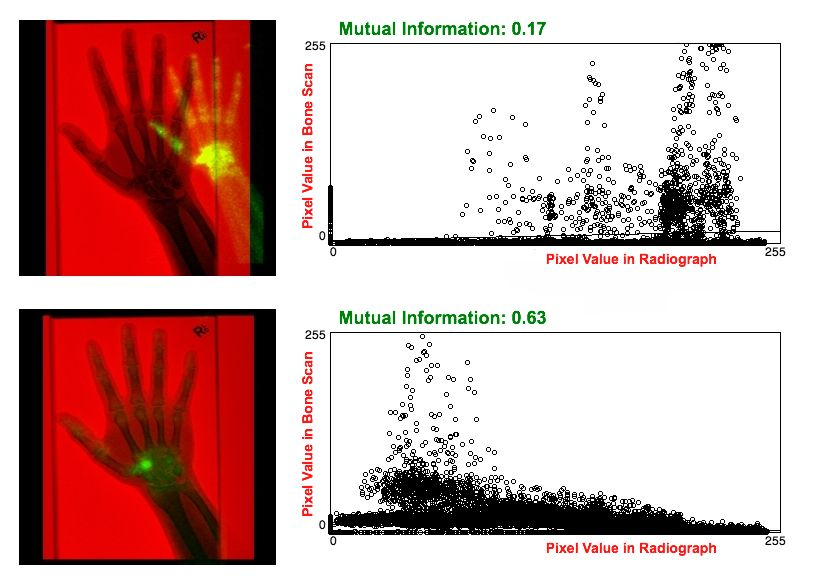
\includegraphics[width=0.9\textwidth]{images/histogramme_conjoint.jpg}\\
\end{column}
\end{columns}
 
\end{frame}
\begin{frame}{Limitation}
\centering
   \begin{columns}[c]
 \begin{column}{0.5\textwidth}
\begin{block}{Hypothèse importante}
\begin{itemize}
  \item Distribution identique dans chaque structure
  \item IRM T1/T2 
  \item CT-CBCT
  \end{itemize}
\end{block}
 \end{column}
 \begin{column}{0.5\textwidth}
\begin{block}{Application HIFU}
\begin{itemize}
  \item Echo/IRM : distributions différentes
  \end{itemize}
\end{block}
\centering
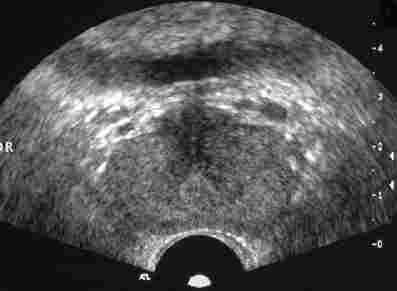
\includegraphics[width=0.4\textwidth]{images/echo_prostate.jpg}
~~~	
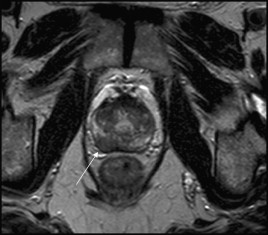
\includegraphics[width=0.4\textwidth]{images/irm_prostate.jpg}
\end{column}
\end{columns}
 
\end{frame}

\subsection{Recalage basé modèle}
\begin{frame}{Entrées}
\centering
   \begin{columns}[c]
 \begin{column}{0.5\textwidth}
\begin{block}{Idée}
\begin{itemize}
  \item Récupérer les contours IRM et echo
  \item Recaler les contours des prostates (ICP)
  \item Appliquer la transformation aux autres contours
  \item Rapide, efficace, mais...
  \end{itemize}
\end{block}
 \end{column}
 \begin{column}{0.5\textwidth}
 \centering
\begin{alertblock}{Problème}
\begin{itemize}
  \item Matrice creuse!
  \item pas de transformation hors contours de la prostate
  \end{itemize}
\end{alertblock}
\end{column}
\end{columns} 
\end{frame}

\begin{frame}{Similarité}
\centering
   \begin{columns}[c]
 \begin{column}{0.5\textwidth}
\begin{block}{Solution}
\begin{itemize}
  \item Recalage des cartes de distances
  \item $\rightarrow$ matrice dense
  \item $\rightarrow$ moins rapide (inversion)
  \item $\rightarrow$ interactions
  \end{itemize}
\end{block}
 \end{column}
 \begin{column}{0.5\textwidth}
 \centering
\begin{exampleblock}{Objectif atteint}
\begin{itemize}
  \item Transfert des informations IRM sur Echo
  \item Visualisation possible en per-opératoire
  \end{itemize}
\end{exampleblock}
\end{column}
\end{columns} 
\end{frame}

\section{Autres applications}
\subsection{Stabilisation de vidéos}
\begin{frame}{Stabilisation}
 
\end{frame}

\subsection{Segmentation basée sur des atlas}
\begin{frame}{Segmentation}
 
\end{frame}
\subsection{Interpolation}
\begin{frame}{Interpolation}
 
\end{frame}


\end{document}
